% Chapter 1

\chapter{Experiments} % Main chapter title

\label{Chapter8}

In this chapter we will display some novel usage in the $ID$ functionalities and qualities.

Here we will use our $ID$ method in order to analyze a problem called image retargeting \cite{}, which is described in blabla's work \cite{}. $ID$ method will apply as a similarity metrics calculator. At last, we will compare its objective images ranking with users ranking the retargeting methods. \\

\textbf{single ID embedding} \ref{Chapter3} will be demonstrated by image classification task


For this section we have used an "image retargeting" dataset \cite{ggg}, which contains a $91$ various images dataset, each image has several attributes such lines/edges, symmetry, faces etc. In this dataset, each several retargeting methods have been applied on every image.

"http://people.csail.mit.edu/mrub/retargetme/"

\begin{figure}[h] \label{rteregt}
	
	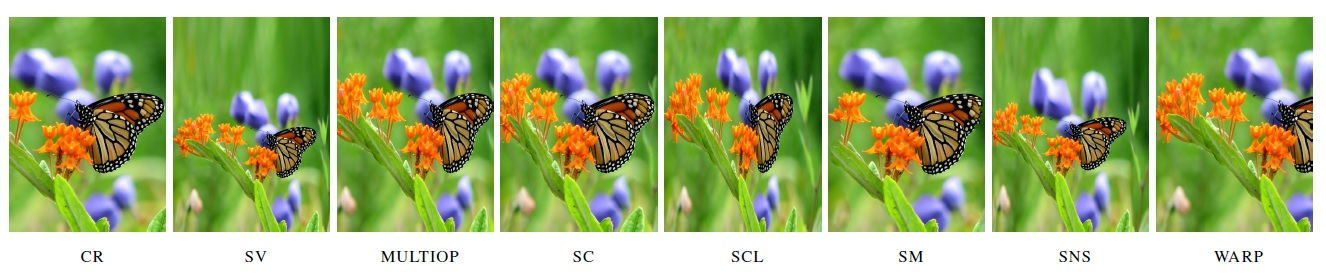
\includegraphics[width=\linewidth,height=12cm,keepaspectratio]{Figures/retargeting}
	\caption[image retargeting example]
	{Example of retargeting the butterfly image to half its size. In this study we evaluate 8 different image retargeting methods, asking users to compare their results and examine what qualities in retargeted images mattered to them. We also correlate the users’ preferences with automatic image similarity measures. Our findings provide insights on the retargeting problem, and present a clear benchmark for future research in the field.}
	
\end{figure}


\section{experiments procedure}

Every image has 8 various retargeting methods. For each image on dataset we have obtained a single vector descriptor. This descriptor is a SIFT descriptor, calculated on the entire image from its center as shown in figure \ref{single_sift}. 
\\ \\ 
Our set is a $n=128$ length dataset, divided to $37$ classes.\\
As described in \ref{Chapter3}, for relatively long vectors such SIFT descriptors, $ID$ method requires memory saving methods. Such method has described in \ref{vbgh} as \textbf{grouping} method. In this method we sample sub-domains from the datasets' vectors, run the $ID$ method separately on each sub-domain, then concatenate the embedded sub-vectors to a flatten embedded vector. \\ 



\begin{figure}[h] \label{single_sift}
	
	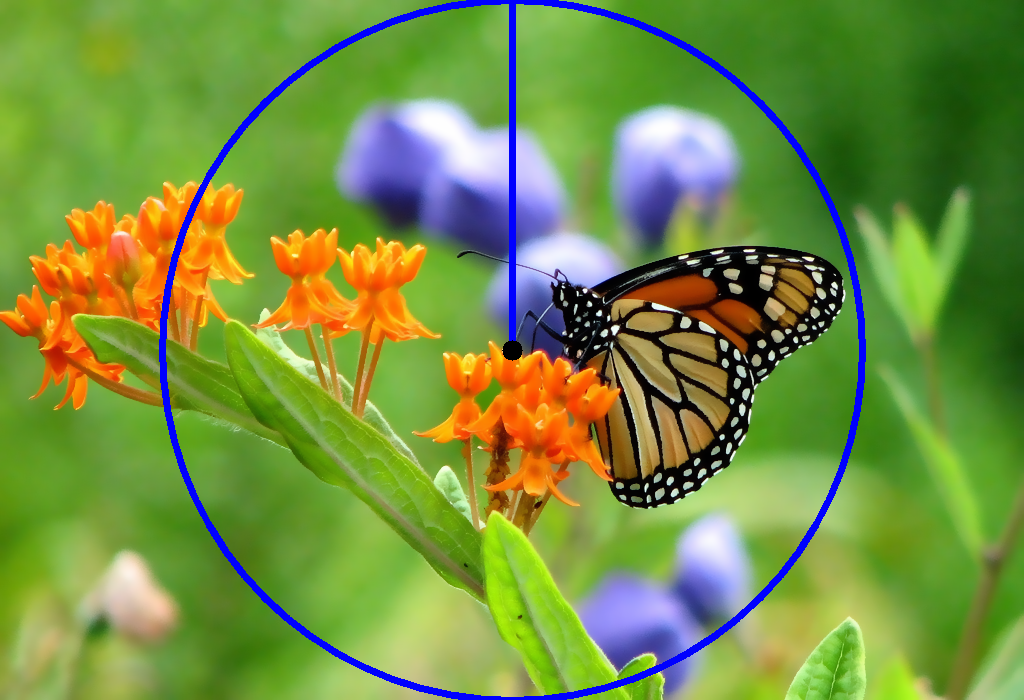
\includegraphics[width=\linewidth,height=12cm,keepaspectratio]{Figures/butterfly_sift}
	\caption[image single sift descriptor]
	{Original butterfly image from retargeting dataset, with an overlay SIFT descriptor on it, as we have measured on every image in the dataset. All SIFT descriptors were taken from the center of the image. Their radius was as the shorter image-side, and their orientation was $+90^{\circ}$.}
	
\end{figure}

The original experiment in the retargeting paper, dealt with ranking comparison, between human perspective, and an objective metrics one. Each metric has ordered its similarity results by ascending order (as described in  \cite{gfdfvdfs}, user votes was sorted by descending order so it may be equivalent to similarity - order).
\\ \\
\textbf{Correlation} was calculated by Kendall-tau correlation distance between users votes and objective metrics similarity ranking results.
\section{Similarity with ID}
Here we have obtained the single objects embedding $ID$ method for similarity analysis. This was performed by applying a SVR \cite{SVR} classifier on embedded single vectors.
SVR model trained on the $37$ reference images, which function as this problem's training set. Problem's test set would be all retargeting method images. Each training-set image was scored (labeled) by an integer score between $[0,36]$. \\

Our test images (which is represented by the embedded vectors) were forwarded by the SVR model, and the absolute distance between the ground truth and its actual score is representing the similarity measure of the certain test image.

\section{parameters}

In our test, the following parameters have been observed:
\begin{itemize}
	\item \textbf{C} - discretization points per dimension. In this particular case we have used a fixed $C$ for all dimensions involved, for simplicity. In general, each dimension may have it's own discretization points number
	\item \textbf{G} - embedded groups number. As described in \ref{grouping} , very long data vectors may consume some serious memory amount through the embedding and learning process, so instead we may use sub-groups of a given dataset. In our case we have sliced-out groups of $4$ elements each. Our grouping method have initiated at the $40^{th}$ element on every SIFT descriptor, and every following group is $4$ elements next.
	\item \textbf{k} - rank size in the comparison between users votes and $ID$ similarity results.
\end{itemize}

SVR model was trained with RBF kernel \cite{rbf}, and $C = 1e5$.
\section{results}

Let us observe the results of $ID$ similarity method with the various parameters. 
As seen in \ref{k-inf} and \ref{k-3}, $ID$ metrics have outperformed almost all previous metrics in terms of correlation ($-1 \leq \tau \leq 1$) between metrics similarity and users correlation votes.


\begin{table}[h]
	\centering
	
	\label{k-inf}
	\resizebox{\textwidth}{!}{
		\begin{tabular}{|c|c|c|c|c|c|c|c|c|c|c|c|}
			\hline
			& \textbf{Lines/Edges} & \textbf{Faces/People} & \textbf{Texture} & \textbf{Foreground Objects} & \textbf{Geometric Structures} & \textbf{Symmetry} & \textbf{Mean} & \textbf{std} & \textbf{p-value} & \textbf{C} & \textbf{G} \\ \hline 	\hline
			\textbf{BDS}      & 0.040 & 0.190   & 0.060  & 0.167   & -0.004    & -0.012   & 0.083  & 0.268  & 0.017 &  &    \\ \hline
			\textbf{BDW}      & 0.031 & 0.048   & -0.048  & 0.060     & 0.004   & 0.119  & 0.046  & 0.181 & 0.869   &   &    \\ \hline
			\textbf{EH}       & 0.043 & -0.076  & -0.060  & -0.079   & 0.103   & 0.298  & 0.004   & 0.334        & 0.641   &   &   \\ \hline
			\textbf{CL}       & -0.023& -0.181  & -0.071  & -0.183   & -0.009     & 0.214   & -0.068  & 0.301  & 0.384  &  &  \\ \hline
			\textbf{RAND}     & -0.046  & -0.014  & 0.048   & -0.032     & -0.040    & 0.143  & -0.031  & 0.284   & 0.693    &  &  \\ \hline
			\textbf{SIFTflow} & 0.097 & 0.252  & 0.119  & 0.218   & 0.085   & 0.071   & 0.145   & 0.262 & 0.031  & & \\ \hline
			\textbf{EMD}      & 0.220 & 0.262  & 0.107  & 0.226   & 0.237    & 0.500  & 0.251  & 0.272  & 1E-5   &  &    \\ \hline
			\textbf{ID\_1}    & 0.42  & 0.42   & 0.40   & 0.43     & 0.42   & 0.41      & 0.42  & 0.013 &   & 6  & 5   \\ \hline
			\textbf{ID\_2}    & 0.45  & 0.44   & \textbf{0.44 }  & 0.43    & 0.41   & 0.44     & 0.44   & 0.014  &    & 6   & 2   \\ \hline
			\textbf{ID\_3}    & \textbf{0.48}  & \textbf{0.49 }    & 0.38    & \textbf{0.46}     & \textbf{0.45}    & \textbf{0.47}   &\textbf{ 0.45 }  & 0.034  &  & 2 & 2 \\ \hline
			\textbf{ID\_4}    & 0.37    & 0.35   & 0.37   & 0.41   & 0.41   & 0.39  & 0.38   & 0.022   &   & 2   & 15  \\ \hline
		\end{tabular}}
		\caption{Complete rank correlation, including new $ID$ results  $(k = \infty)$}
	\end{table}
	
	
	
	\begin{table}[h]
		\centering
		
		\label{k-3}
		\resizebox{\textwidth}{!}
		{\begin{tabular}{|c|c|c|c|c|c|c|c|c|c|c|c|}
				\hline
				& \textbf{Lines/Edges} & \textbf{Faces/People} & \textbf{Texture} & \textbf{Foreground Objects} & \textbf{Geometric Structures} & \textbf{Symmetry} & \textbf{Mean} & \textbf{std} & \textbf{p-value} & \textbf{C} & \textbf{G} \\ \hline
				\textbf{BDS}      & 0.062  & 0.280     & 0.134    & 0.249    & -0.025  & -0.247  & 0.108   & 0.532   & 0.005   &   &     \\ \hline
				\textbf{BDW}      & 0.213 & 0.141     & 0.123    & 0.115     & 0.212   & 0.439    & 0.200   & 0.395   & 0.002 &  & \\ \hline
				\textbf{EH}       & -0.036    & -0.207    & -0.331    & -0.177   & 0.111     & 0.294  & -0.071  & 0.593  & 0.013   &  & \\ \hline
				\textbf{CL}       & -0.307    & -0.336  & -0.433    & -0.519      & -0.366     & 0.088   & -0.320   & 0.543  & 1E-6    &   &     \\ \hline
				\textbf{RAND}     & 0.241  & 0.428  & 0.312     & 0.442     & 0.303    & 0.002   & 0.298  & 0.483  & 1E-6    &   &    \\ \hline
				\textbf{SIFTflow} & 0.301    & 0.416   & 0.216    & 0.295    & 0.226   &\textbf{ 0.534 }  & 0.326   & 0.496   & 1E-6      &   &   \\ \hline
				\textbf{EMD}      & 0.220    & 0.262    & 0.107   & 0.226     & 0.237   & 0.500   & 0.251   & 0.272  & 1E-5     &    &     \\ \hline
				\textbf{ID\_1}    & 0.41  & 0.42 & 0.41     &\textbf{ 0.48 }  &\textbf{ 0.56 } & 0.46    & 0.46    & 0.051  &   & 6    & 5  \\ \hline
				\textbf{ID\_2}    &\textbf{ 0.48}   & \textbf{0.50 } & \textbf{0.43  }  & \textbf{0.48  }   & 0.46   & 0.46   &\textbf{ 0.47 }  & 0.022  &    & 6  & 2  \\ \hline
				\textbf{ID\_3}    &\textbf{ 0.48 }     & \textbf{0.50}    & 0.39    & 0.42   & 0.38     & 0.44    & 0.43   & 0.045   &   & 2     & 2     \\ \hline
				\textbf{ID\_4}    & 0.46     & 0.42  & 0.35     & 0.38   & 0.46     & 0.39   & 0.41     & 0.041  &   & 2      & 15   \\ \hline
			\end{tabular}}
			
			\caption{Rank correlation with respect to the three highest rank results, including new $ID$ $(k = 3)$} 
		\end{table}
		
		
This basic fact verifies our correctness of our multidimensional $ID$ embedding method, as well as its sub-sampling grouping method for memory saving.
As described in \cite{retargeting}, SIFTflow \cite{siftflow} and EMD \cite{EMD} both relies on spatial descriptors, which may be most similar to human eye-brain interpretations of a difference/similarity among pairs of images. The advantage of our method is the ability to magnify differences among data elements by the applying an embedding process which divides the data into $C$ groups per dimension, so a difference between 2 data elements may only get larger ( or at least stay as the original data elements) since it may separate data elements into several different simplices, and by that embed them into totally different locations on the embedded vector. \\
		
		%-------------------------------------------------------------------------------------
		
		\begin{figure}[h] \label{bf_id}
			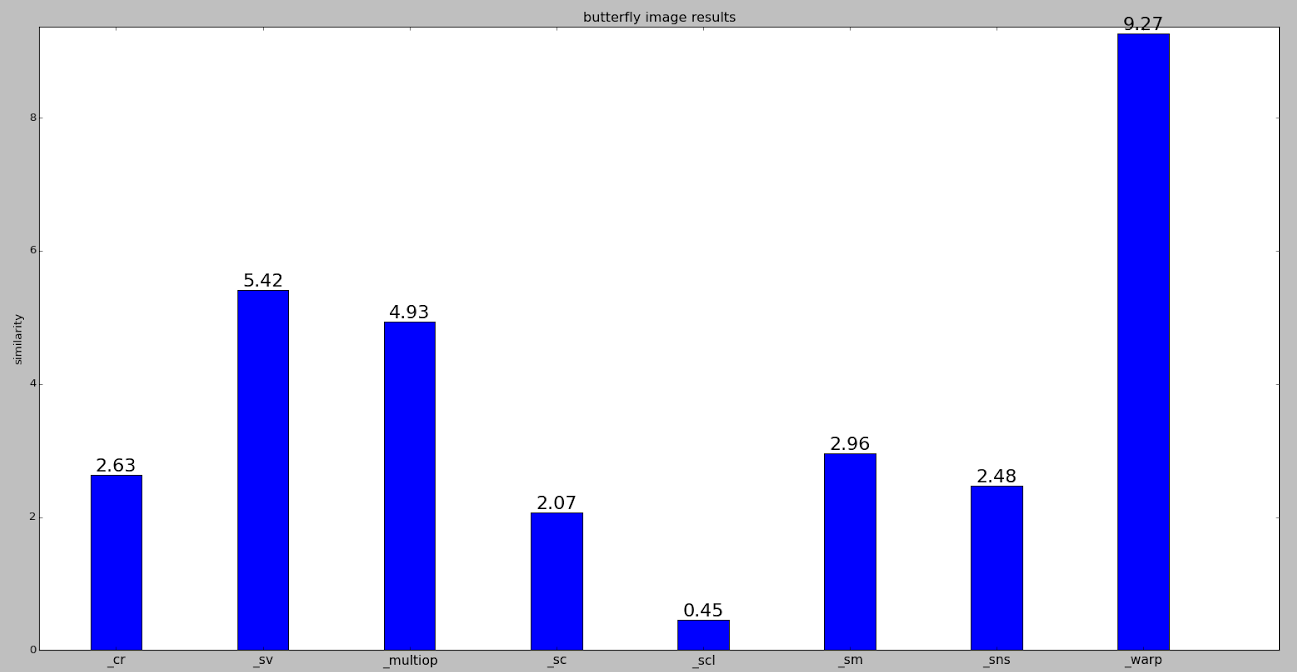
\includegraphics[width=\linewidth,height=12cm,keepaspectratio]{Figures/bf_id}
			\caption[butterfly similarity results]
			{butterfly similarity results}
		\end{figure}
		
		\begin{figure}[h] \label{bf_usr}
			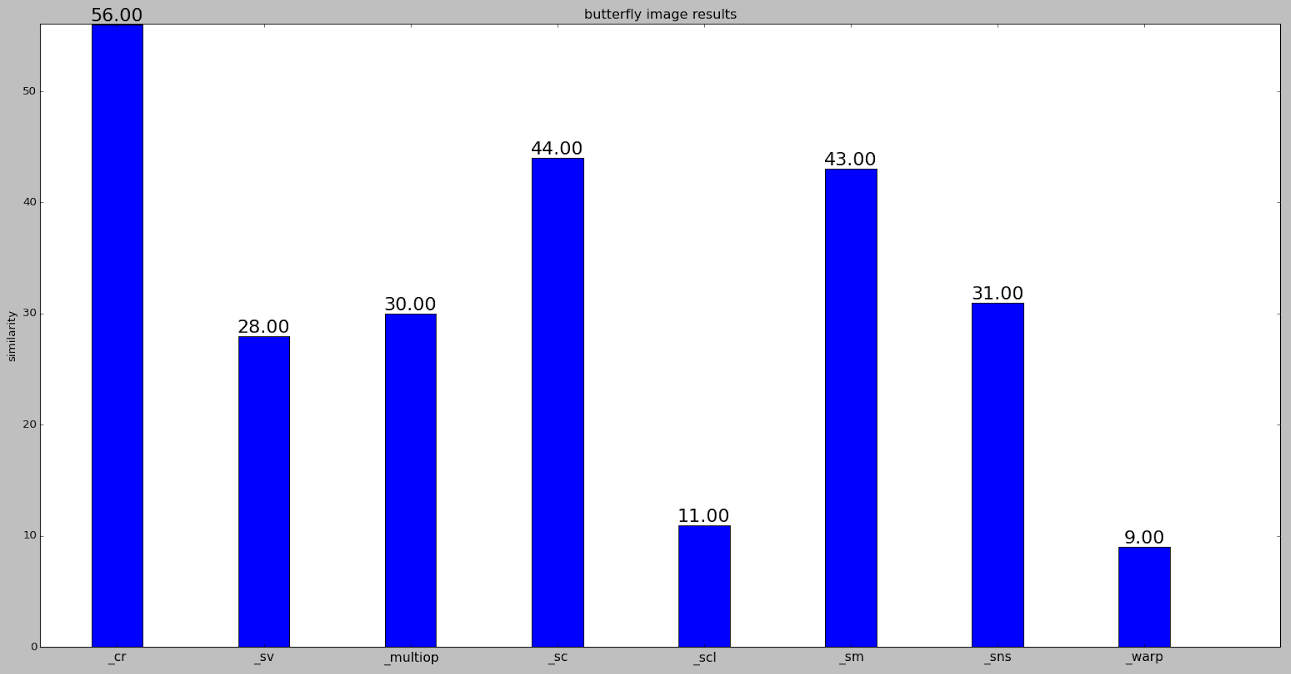
\includegraphics[width=\linewidth,height=12cm,keepaspectratio]{Figures/bf_usr}
			\caption[butterfly similarity users votes]
			{butterfly similarity users votes}
		\end{figure}
		
In figures \ref{bf_id},\ref{bf_usr}, we demonstrate $ID$ similarity results on the butterfly image \ref{single_sift}, in comparison to the users votes. As seen on the similarity graph, some retargeting methods such warp \cite{warp} may have not that good similarity result in relation to the reference image, but in this scenario we observed the relative results of the ranking of all methods between users votes and our $ID$ metric.
		
		%-------------------------------------------------------------------------------------
		
		\begin{figure}[h] \label{c2g2k3}
			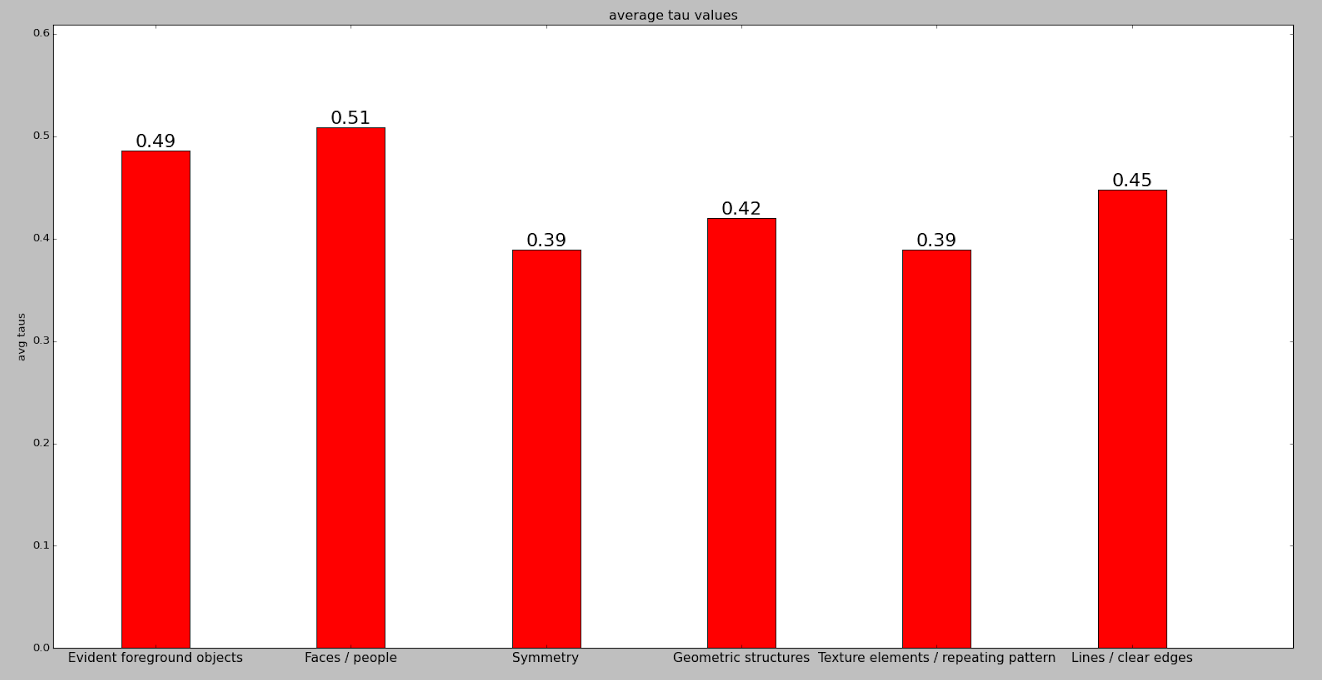
\includegraphics[width=\linewidth,height=12cm,keepaspectratio]{Figures/c2g2k3}
			\caption[C = 2 , G = 2 , k = 3]
			{C = 2 , G = 2 , k = 3}
		\end{figure}
		
		\begin{figure}[h] \label{c2g2kinf}
			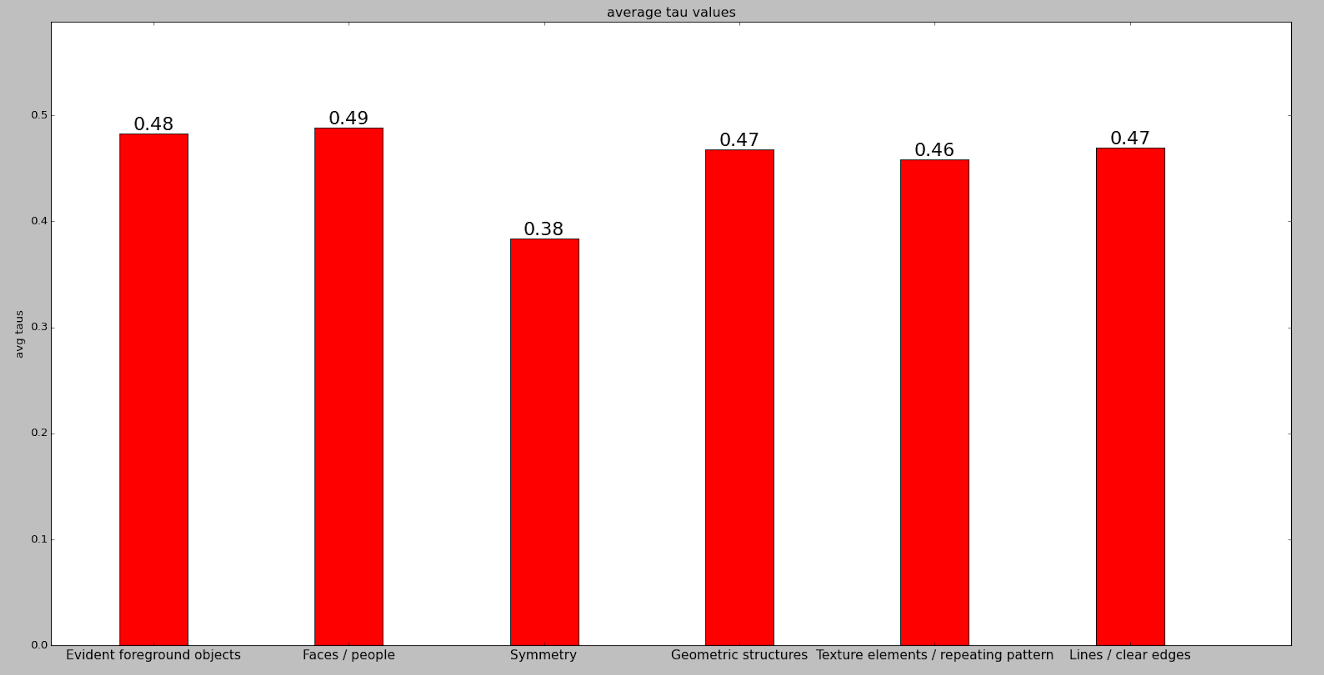
\includegraphics[width=\linewidth,height=12cm,keepaspectratio]{Figures/c2g2kinf}
			\caption[c2g2kinf]
			{c2g2kinf}
		\end{figure}
		
		%-------------------------------------------------------------------------------------
		
		\begin{figure}[h] \label{c6g2k3}
			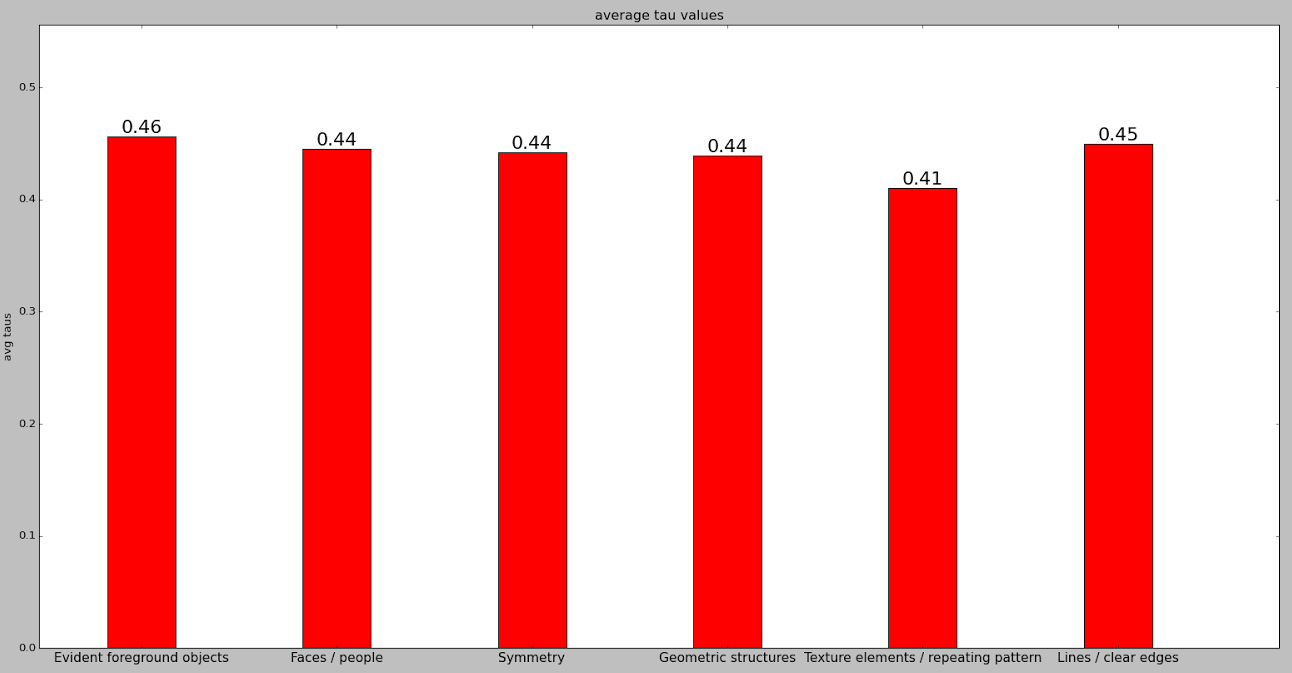
\includegraphics[width=\linewidth,height=12cm,keepaspectratio]{Figures/c6g2kinf}
			\caption[c6g2kinf]
			{c6g2kinf}
		\end{figure}
		
		\begin{figure}[h] \label{c6g2kinf}
			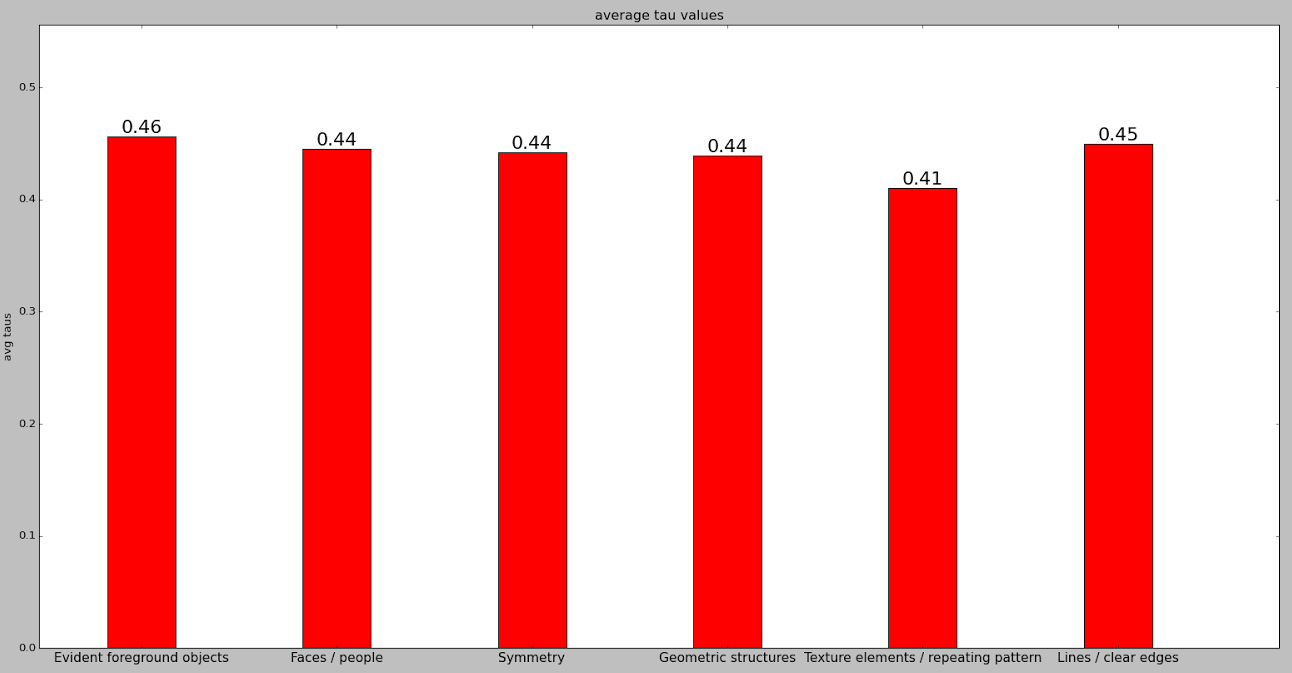
\includegraphics[width=\linewidth,height=12cm,keepaspectratio]{Figures/c6g2kinf}
			\caption[c6g2kinf]
			{c6g2kinf}
		\end{figure}
		
		
		%-------------------------------------------------------------------------------------
		
		\begin{figure}[h] \label{c6g5k3}
			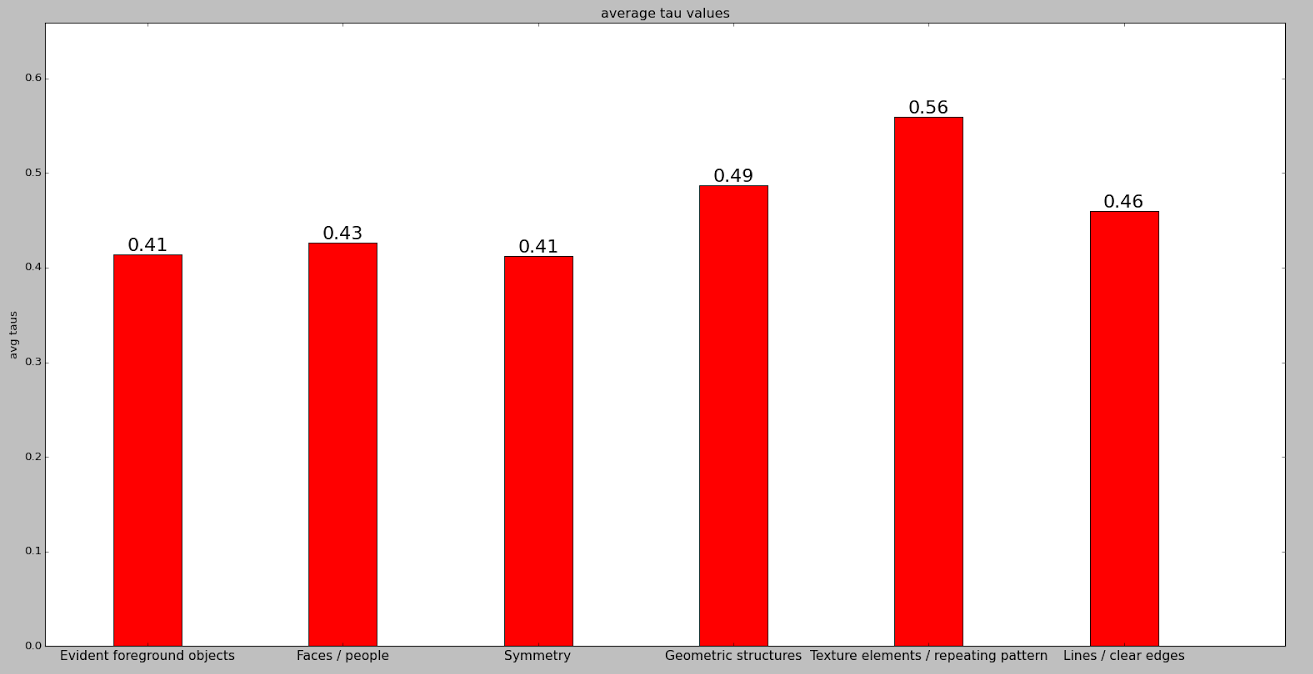
\includegraphics[width=\linewidth,height=12cm,keepaspectratio]{Figures/c6g5k3}
			\caption[c6g5k3]
			{c6g5k3}
		\end{figure}
		
		\begin{figure}[h] \label{c6g5kinf}
			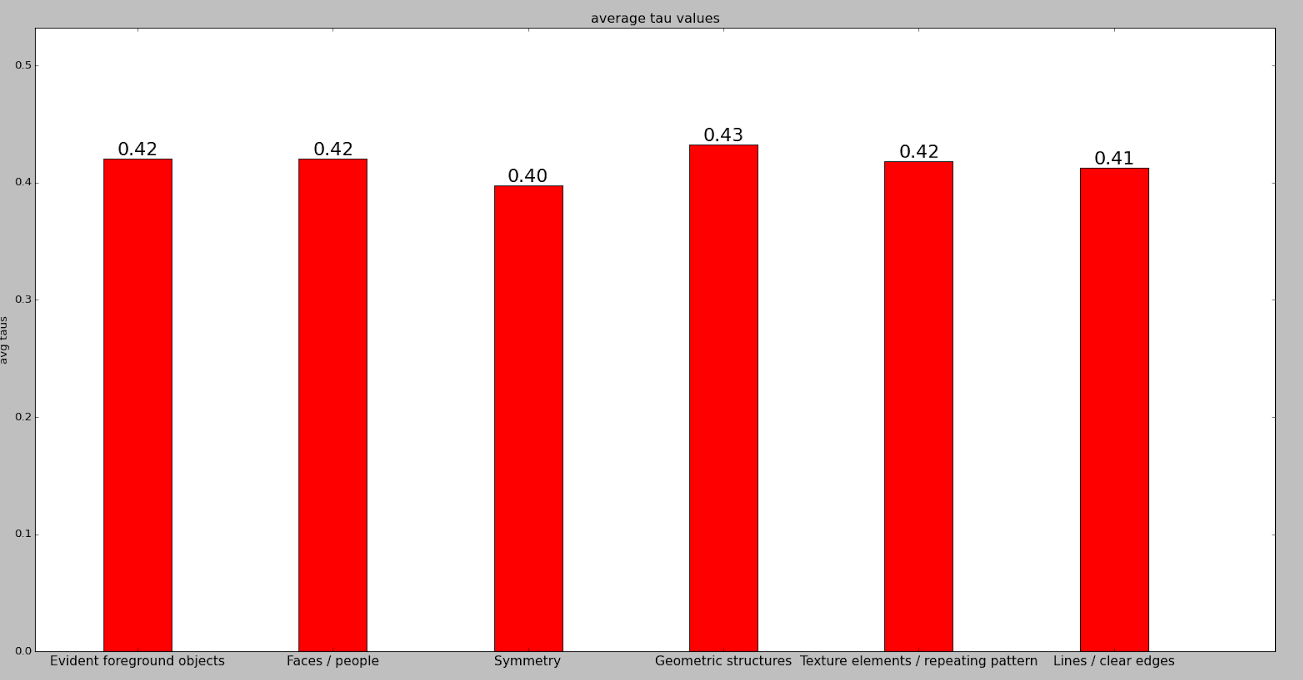
\includegraphics[width=\linewidth,height=12cm,keepaspectratio]{Figures/c6g5kinf}
			\caption[c6g5kinf]
			{c6g5kinf}
		\end{figure}
		
	
		%-------------------------------------------------------------------------------------
		
		\begin{figure}[h] \label{c2g15k3}
			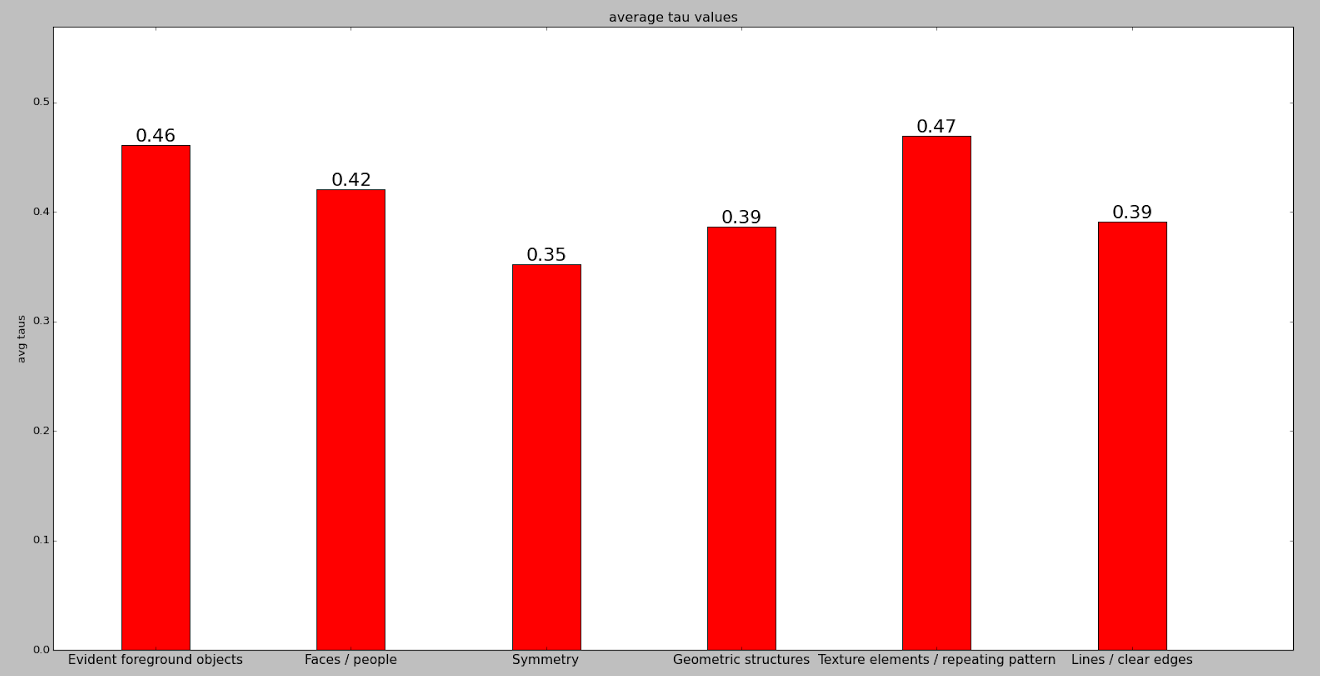
\includegraphics[width=\linewidth,height=12cm,keepaspectratio]{Figures/c2g15k3}
			\caption[c2g15k3]
			{c2g15k3}
		\end{figure}
		
		\begin{figure}[h] \label{c2g15kinf}
			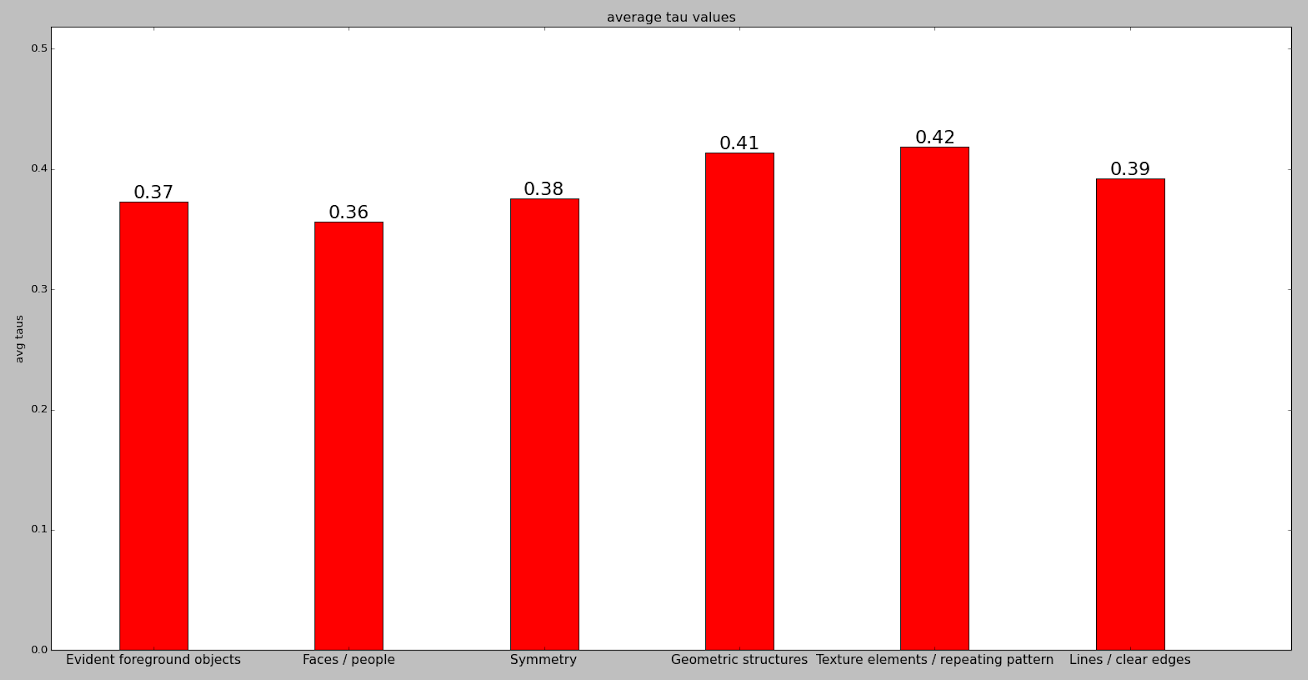
\includegraphics[width=\linewidth,height=12cm,keepaspectratio]{Figures/c2g15kinf}
			\caption[c2g15kinf]
			{c2g15kinf}
		\end{figure}
